\section{Tasks}
\subsection{Overview}
In this chapter we will provide an overview of the tasks and how we will divide them within the group. \\
We will do a simply overview of the Macro-tasks and we'll create a Gantt chart to make this section simple and clear because the graph will be self explanatory.\\
The COCOMO II overview gave the resoult of about ~3,6 months, so our schedule will start the 1 of october and will finish before the end of January.
\subsection{MacroTasks}
\subsubsection{RASD}
The initial phase will be the creation of the RASD to describe the system in terms of functional and nonfunctional requirements, it  will be a contractual base between the customer and the developing. 

\subsubsection{Design}
We will write the Design Document, working on the Components of the application, the database projecting and the deployment and run-time definition.

\subsubsection{Test Plan}
We will then study our project and start thinking about objectives, target market, processes for a specific beta test for the software.

\subsubsection{Project Making}
This is the main phase of the project, we will build the application and whatever concerns it's work, Following the steps of the ProjectPlan and the other phases.

\subsubsection{Final Tests}
As descripted in the Test plan documents, there will be a phase of testing and even implementations to be sure that everything works fine in every situation.

\newpage
\begin{landscape}
   \begin{figure}[ht]
    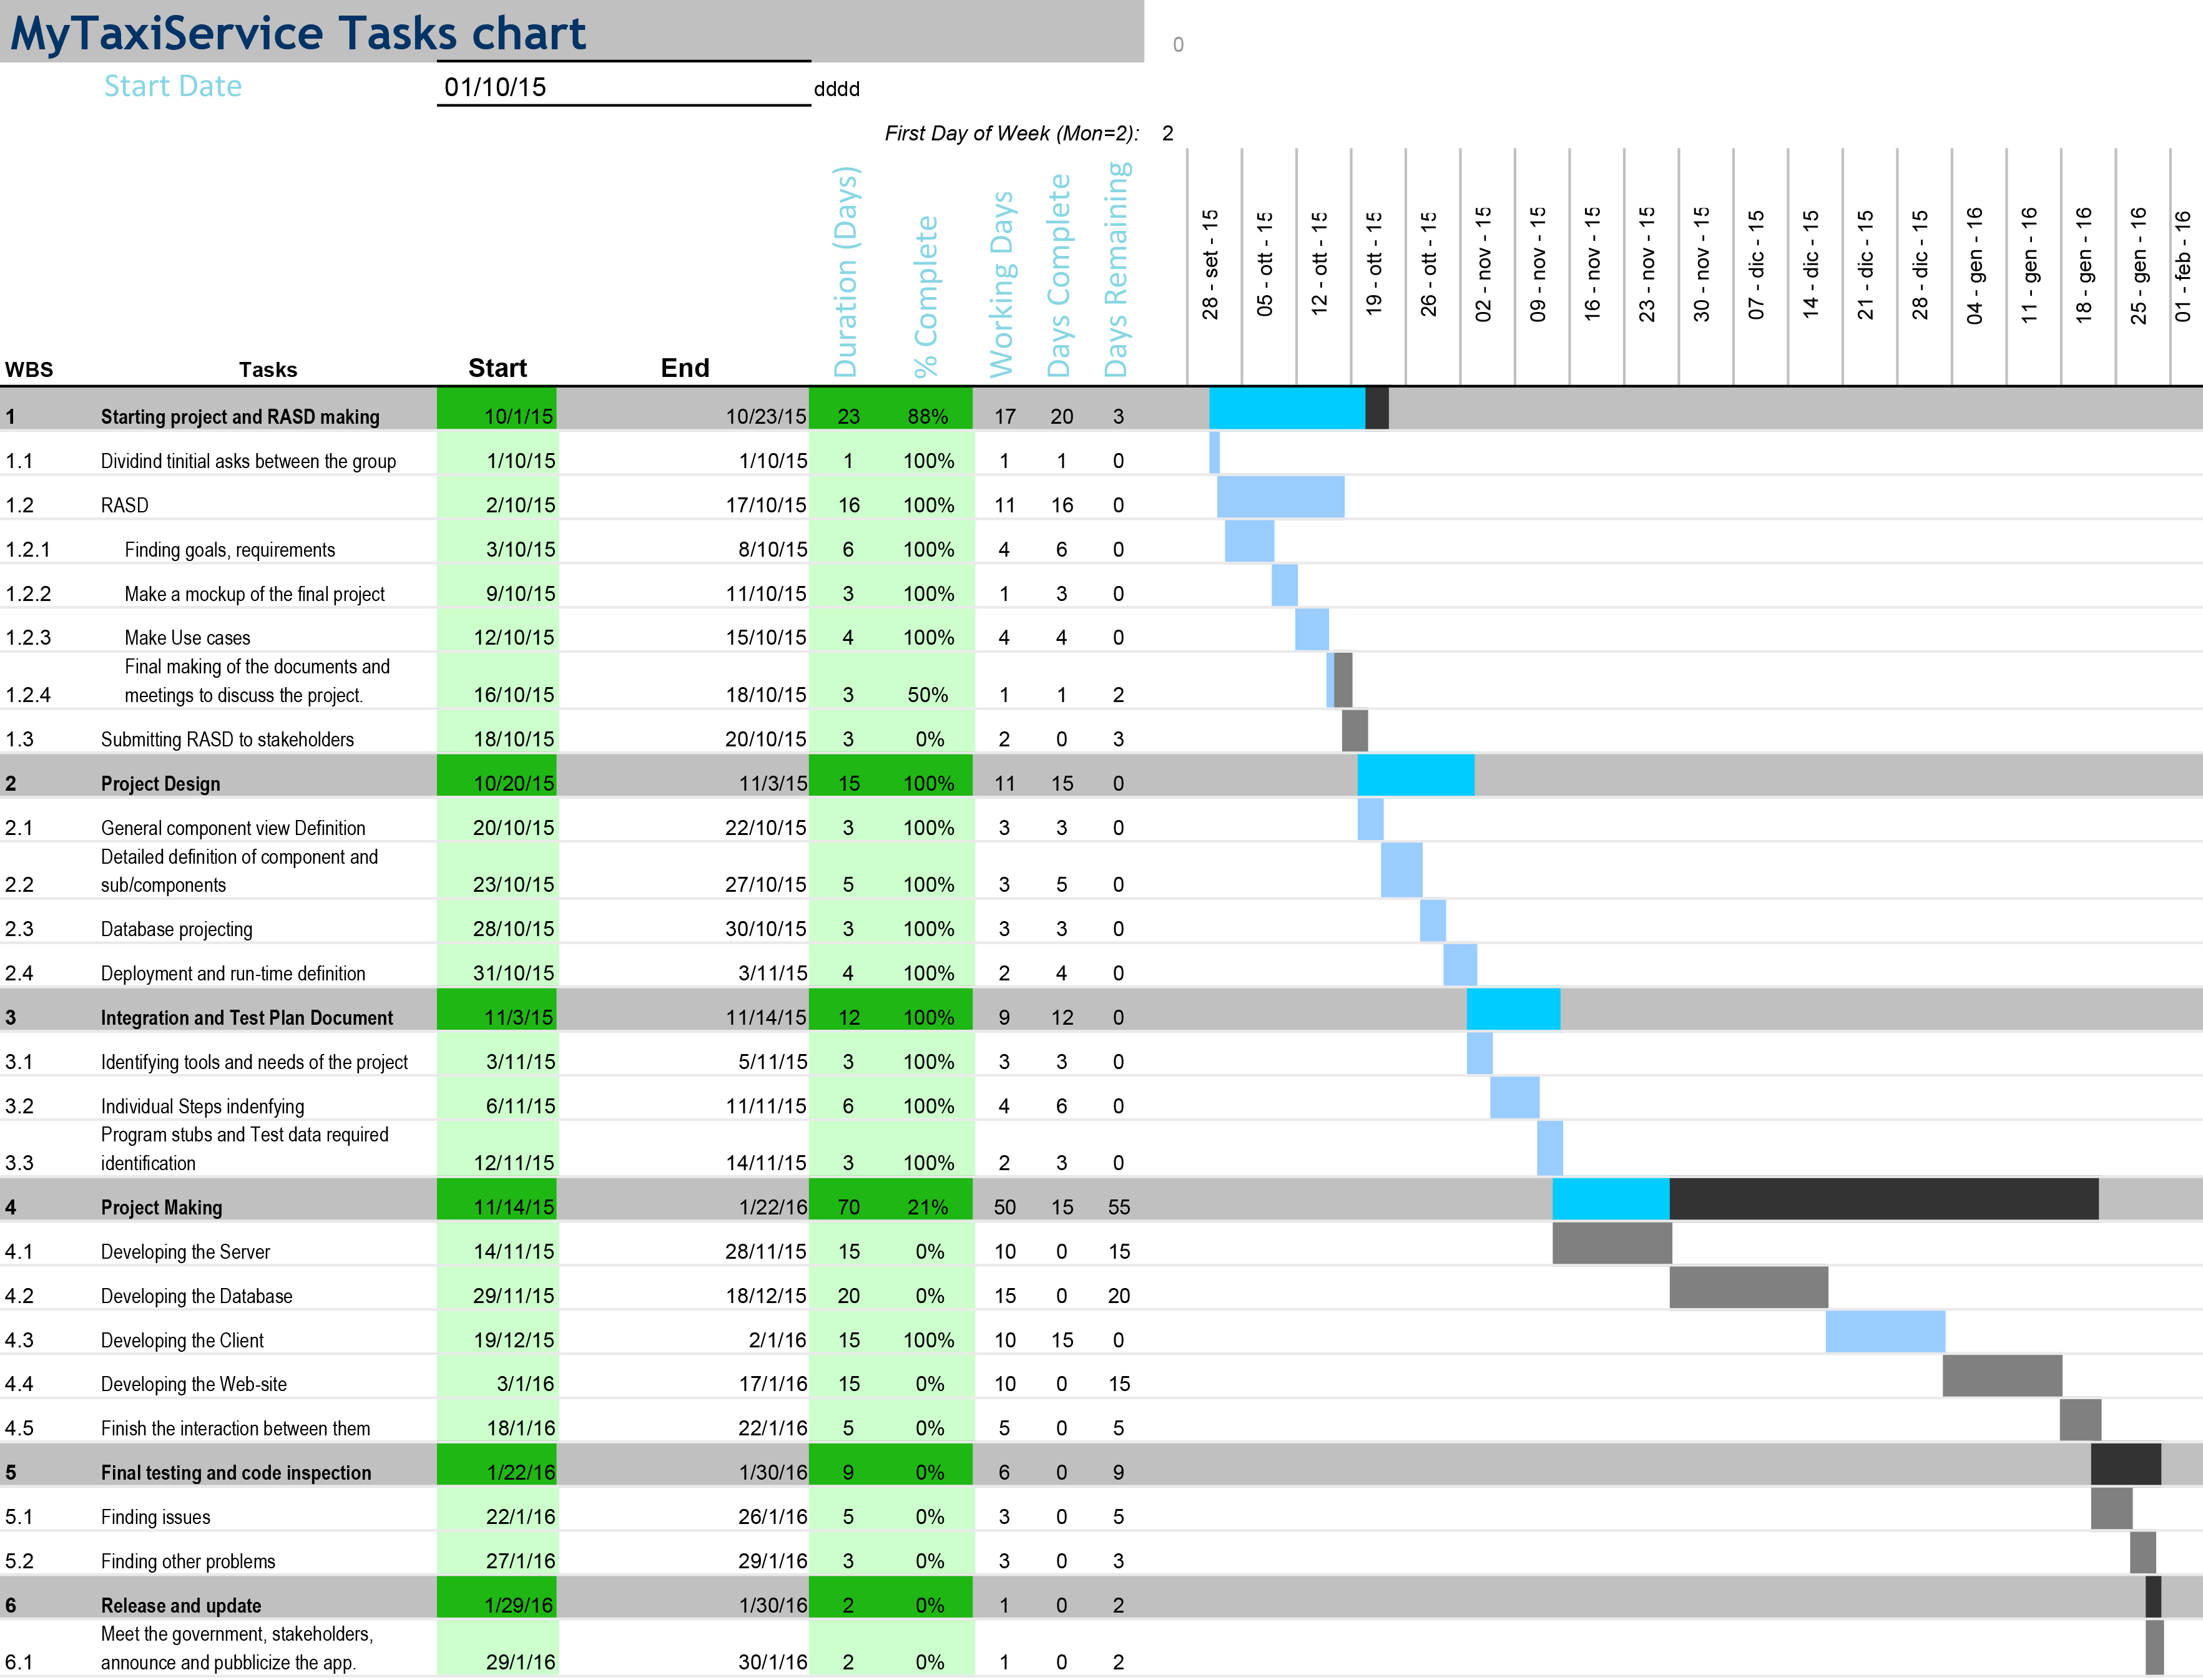
\includegraphics[width=1.5\textwidth]{akjfserljgiehksrghlkjserh.png}
    
    \caption{Gantt Chart}
    \label{fig: Gantt Chart}
	\end{figure}

           \end{landscape}
